\documentclass[a4paper, fontsize=12pt, parskip=half]{scrartcl}
\usepackage{float}
\usepackage[utf8]{inputenc}
\usepackage[T1]{fontenc}
\usepackage{textcomp}
\usepackage[brazil]{babel}
\usepackage[portuguese,algoruled,longend]{algorithm2e}
\usepackage{algorithmic}
\usepackage{amsmath,amssymb,amsthm,textcomp}
\usepackage{float}
\usepackage{graphicx}

\newtheoremstyle{mytheor}
{1ex}{1ex}{\normalfont}{0pt}{\scshape}{.}{1ex}
{{\thmname{#1 }}{\thmnumber{#2}}{\thmnote{ (#3)}}}

\theoremstyle{mytheor}
\newtheorem{defi}{Definição}
\newtheorem{teorema}{Teorema}
\newtheorem{corolario}{Corolário}


% for matlab code
% bw = blackwhite - optimized for print, otherwise source is colored
\usepackage[framed,numbered,bw]{mcode}

% for other code
%\usepackage{listings}

\setlength{\parindent}{0em}

% set section in CM
\setkomafont{section}{\normalfont\bfseries\Large}

\newcommand{\mytitle}[1]{{\noindent\Large\textbf{#1}}}
\newcommand{\mysection}[1]{\textbf{\section*{#1}}}
\newcommand{\mysubsection}[2]{\romannumeral #1) #2}


%===================================
\begin{document}

\noindent\textbf{Instituto de Computação -- IComp} \hfill \textbf{Universidade Federal do Amazonas}\\
Aluno: Ruan Gabriel Gato Barros \hfill Matrícula: 21553690\\
Professor: Raimundo Barreto \hfill \\

\mytitle{TP9 e TP10 - Multithreading}\\\\
%===================================

\section{Configuração da Máquina}

Os experimentos foram executadas em uma máquina que utilizava um processador \texttt{Intel Core i5-4200U} e sistema operacinal \texttt{Linux Mint 18.1}

\begin{lstlisting}
processor	: 0
vendor_id	: GenuineIntel
cpu family	: 6
model		: 69
model name	: Intel(R) Core(TM) i5-4200U CPU @ 1.60GHz
stepping	: 1
microcode	: 0x1c
cpu MHz		: 2300.089
cache size	: 3072 KB
physical id	: 0
siblings	: 4
core id		: 0
cpu cores	: 2
apicid		: 0
initial apicid	: 0
fpu		: yes
fpu_exception	: yes
cpuid level	: 13
wp		: yes
bogomips	: 4589.26
clflush size	: 64
cache_alignment	: 64
address sizes	: 39 bits physical, 48 bits virtual
\end{lstlisting}

\section{Exercicio 1 - Variável global}
Nesse exercício, executei soma de um vetor de \textit{n} posições geradas aleatóriamente, sendo essa soma compartilhada por \textit{p} \textit{threads}, cada \textit{thread} compartilhando um range de execução das somas, todas compartilhando a mesma variável, utilizando para isso, uma exclusão mútua nessa condição de corrida \texttt{(mutex)}.

\begin{figure}[htb!]
	\centering
	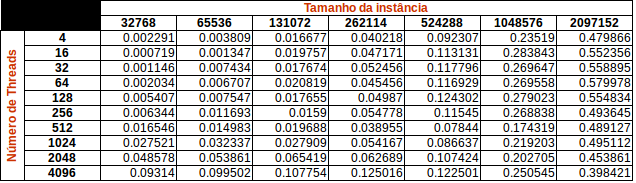
\includegraphics[width=1\linewidth]{gfx/1aQ}
	\caption{Tabela dos tempos de execução do exercício 1}
	\label{fig:1aq}
\end{figure}

\begin{figure}[htb!]
	\centering
	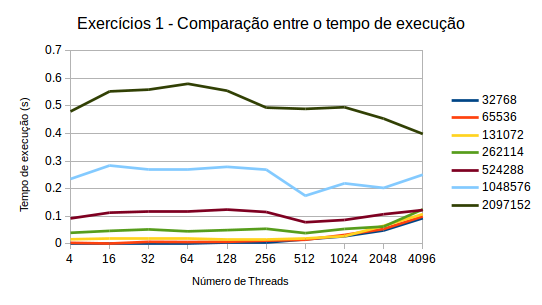
\includegraphics[width=1\linewidth]{gfx/1aQ_g}
	\caption{Grafico dos tempos de execução do exercício 1}
	\label{fig:1aq_g}
\end{figure}

\section{Exercicio 2 - Vetor auxiliar}
O experimento foi realizado de maneira análoga ao exercício 1, porém, ao invés de uma variável global, cada \textit{thread} responderia por uma posição em um novo vetor com o número de \textit{threads} em posições.
\begin{figure}[htb!]
	\centering
	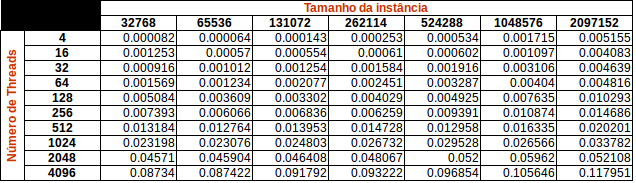
\includegraphics[width=1\linewidth]{gfx/2aQ}
	\caption{Tabela dos tempos de execução do exercício 2}
	\label{fig:2aq}
\end{figure}

\begin{figure}[htb!]
	\centering
	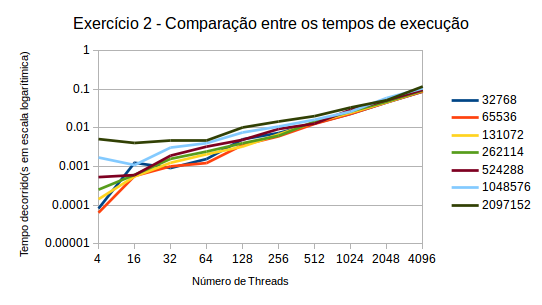
\includegraphics[width=1\linewidth]{gfx/2aQ_g}
	\caption{Grafico dos tempos de execução do exercício 2}
	\label{fig:2aq_g}
\end{figure}

\section{Exercicio 3 - Variável local}
De maneira equivalente ao exercício 2, as \textit{threads} agora não guardarão a soma em um novo vetor, e sim em uma variável local; o objetivo dessa técnica é não utilizar locks na atualização das variáveis, e, com isso, tentar ganhar algum desempenho no que diz respeito à não-inclusão de processamento extra das exclusões mútuas.\\
\begin{figure}[htb!]
	\centering
	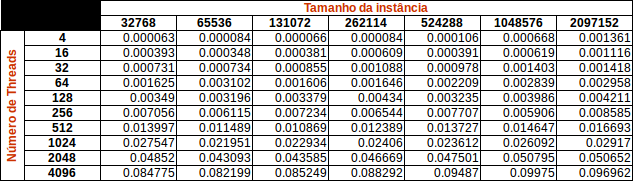
\includegraphics[width=1\linewidth]{gfx/3aQ}
	\caption{Tabela dos tempos de execução do exercício 3}
	\label{fig:3aq}
\end{figure}

\begin{figure}[htb!]
	\centering
	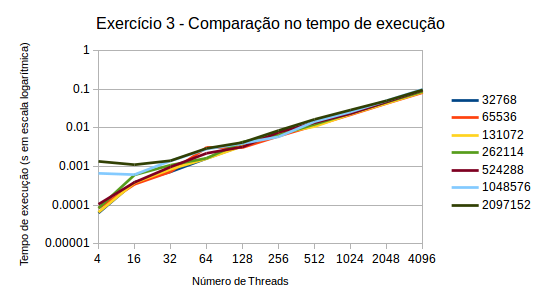
\includegraphics[width=1\linewidth]{gfx/3aQ_g}
	\caption{Grafico dos tempos de execução do exercício 3}
	\label{fig:3aq_g}
\end{figure}

\section{Exercicio 4 - Comparação}

\subsection{Exercício 1 \textit{in a nutshell}}

No que diz respeito ao primeiro exercício, ele foi o pior caso de execução, uma vez que a utilização da trava de exclusão mútua seria muito disputada por todas as \textit{threads}, o que acarretaria em uma degeneração na execução das \textit{threads} que não conseguiram o acesso ao lock no instânte, ou seja, para 1000 \textit{threads}, 1 conseguia executar verdadeiramente e 999 ficaram esperando. 

Com um número pequeno de \textit{threads}, mais trabalho cada uma teria individualmente, por isso, quanto maior o número de \textit{threads}, menor seria o tempo de execução invididual de cada uma, consequentemente diminuiria mais rápido a disputa pelo lock, o que explica a melhora no tempo de execução à partir de 256 \textit{threads} na instância de 2048K.

\subsection{Exercício 2 \textit{in a nutshell}}

No exercício 2, não se fez necessário o uso de uma trava de exclusão mútua, o que fez o desempenho melhorar em relação ao exercício 1, já que a disputa pelo vetor auxiliar seria somente de leitura, tornando desnecessário o uso dessa trava. A grande desvantagem desse exercício em contraste com o exercício 3 é o fato de precisar realizar cálculo de posições de memória ao acessar o vetor, por exemplo, a \textit{thread} 3 que será responsável pelas posições 50 a 150 do vetor terá que calcular $\&vetor (endereço\_inicial\_do\_vetor) + numeroThread$ para recuperar a posição do vetor auxiliar que lhe diz respeito, para só assim realizar cálculos.

\subsection{Exercício 3 \textit{in a nutshell}}
De fato, o exercício 3 se mostrou o melhor entre os três, uma vez que a utilização da variável local para cara \textit{thread} torna o processamento extra de calcular a posição do vetor em todo loop desnecessário, o que melhora potencialmente o tempo de execução, como é possível averiguar nas tabelas de tempo de execução. Em contraste com o exercício 2, o exercício 3 possui melhor tempo justamente por esse artifício, uma operação de soma a mais a cada iteração do loop no exercício 2 pôde degenerar o tempo de execução.

\section{Exercício 5 \& Exercício 6 - QuickSort vs QuickSort Paralelo (versão Näive)}

O \textit{quicksort} utiliza a estratégia divisão e conquista em sua execução e possui uma solução bem simples recursiva.

Em implementações iterativas é necessário implementar uma pilha de execuções de ponteiros de funções e parâmetros, simulando o que parece ser uma máquina virtual de pilhas que, mesmo possuindo funcionamento mais complexo que sua versão recursiva, é bastante eficiente. 

Porém, nesse exercício comparei a versão recursiva do \textit{quicksort} com a versão recursiva do \textit{quicksort} paralelo, que, para minha surpresa, teve resultados bem desapontadores.\\\\

\begin{figure}[htb!]
	\centering
	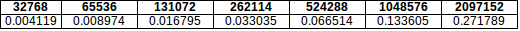
\includegraphics[width=1\linewidth]{gfx/5aQ}
	\caption{Exercício 5 - Tempo de execução do QuickSort Recursivo}
	\label{fig:5aq}
\end{figure}

\begin{figure}[htb!]
	\centering
	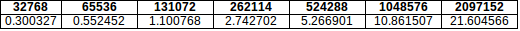
\includegraphics[width=1\linewidth]{gfx/6aQ}
	\caption{Exercício 6 - Tempo de execução do QuickSort Recursivo Paralelo}
	\label{fig:6aq}
\end{figure}

\begin{figure}[htb!]
	\centering
	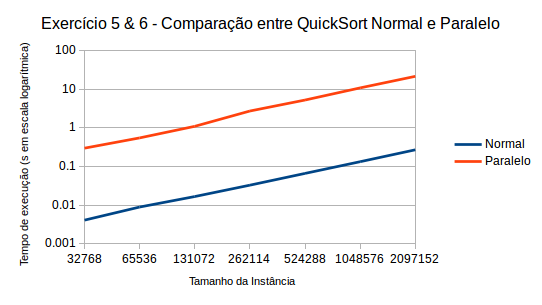
\includegraphics[width=1\linewidth]{gfx/56aQ_g}
	\caption{Exercício 6 - Comparação do Tempo de execução do QuickSort Recursivo e Recursivo Paralelo}
	\label{fig:56aq}
\end{figure}


\subsection{Discussão sobre os tempos de execução}

No que diz respeito à implementação, a segunda metade da execução está sendo tratada como uma nova thread; mesmo que a primeira fosse tratada como uma nova thread, ainda seria necessário travar a execução à espera do término da thread para que o nível mais alto consiga executar seu processamento de forma correta, isso faz com que o número de threads criadas até o final da árvore de recursões ser atingido seja proporcional ao número de partições desde a raiz até a última folha, tendo assim um número enorme de concorrências por recursos computacionais acontecendo em diferentes níveis, oque torna a execução impraticável, uma vez que seria muito menos custoso somente esperar pelo término da execução da \textit{stack}. 

Como é possível ver, na instância de 32K já é notável o aumento significativo no tempo de execução, sendo a proporção de tempo do \textit{quicksort} paralelo em relação ao \textit{quicksort} normal em média 70x maior, tornando-o 70x mais demorado.

Outra anomalia detectada foi em relação à entropia de espalhamento do vetor inicial, quanto menor ordenado o vetor, mais problemas causava para o quicksort paralelo, uma vez que cada thread tomaria muito mais tempo que o esperado trocando posições em relação ao pivot.

\end{document}